% JINST-style manuscript (mimics the JINST layout; jinst.cls not required).
% Topic: agent-assisted provenance of the ATLAS & CMS Run-2 Delphes cards.
\documentclass[11pt,a4paper]{article}

\usepackage[margin=2.4cm]{geometry}
\usepackage{amsmath}
\usepackage{array}
\usepackage{booktabs}
\usepackage{longtable}
\usepackage{graphicx}
\usepackage{float}
\usepackage[hidelinks]{hyperref}
\usepackage{xcolor}

\newcommand{\eqA}{\sigma(p_\mathrm{T})/p_\mathrm{T}=\sqrt{a^2+(b\,p_\mathrm{T})^2}}
\newcommand{\flag}[1]{\textcolor{black}{\textsf{#1}}}
\setlength{\parskip}{3pt}

\title{\bf Toward citable, uncertainty-aware Delphes cards:\\
an agent-assisted provenance audit of the ATLAS and CMS Run-2 parameterizations}
\author{B.~Nachman \emph{et al.}\\[2pt]
\small (manuscript draft --- generated with an AI-agent provenance pipeline)}
\date{\today}

\begin{document}
\maketitle

\begin{abstract}
\noindent
The widely used fast-simulation framework \textsc{Delphes} models detector
response through hard-coded parameterizations --- tracking and identification
efficiencies, momentum and energy resolutions, jet-energy scale, and
flavour-tagging rates --- that are distributed in plain-text ``cards.'' For the
reference ATLAS and CMS Run-2 cards the overwhelming majority of these numbers
carry \emph{no citation} and \emph{no uncertainty}, so a user cannot trace a
given value to a measurement or propagate its error. We report a systematic
provenance audit of the two cards in which every measured parameterization is
mapped to an authoritative public source, the value is extracted with its
locator (table/figure/equation) and uncertainty, and each extraction is
re-checked by an \emph{independent adversarial verifier} before it is accepted.
The audit is executed as a multi-agent pipeline: $26$ parameter blocks
(\textasciitilde$140$ individual coefficients) were source-mapped, extracted,
and verified. We find that while several blocks are already consistent with the
literature (notably the ATLAS electromagnetic-calorimeter resolution and the
b-tagging working points), a large fraction --- about $88$ coefficients --- are
not: the charged-hadron track-momentum resolution is too pessimistic in both
experiments by a factor $\sim\!3$ at high $p_\mathrm{T}$ (slope-dominated) rising
to $\sim\!6$--$12$ at low $p_\mathrm{T}$ (the constant term), the electron
``momentum'' resolution is
modelled with the wrong (tracker-like) functional form for a
calorimeter-dominated measurement, and several tracking/identification
efficiency plateaus are optimistic by $5$--$10\%$ absolute. We release the full
machine-readable provenance, propose source-faithful baseline values with
uncertainties, and outline the path to citable \texttt{*\_baseline} and
\texttt{*\_uncertainty} cards suitable for systematic studies.
\end{abstract}

\section{Introduction}
\textsc{Delphes}~\cite{delphes} parameterizes detector response rather than
simulating it microscopically, which makes it the standard tool for phenomenology
and for experimental sensitivity projections. The fidelity of a \textsc{Delphes}
study rests entirely on the numbers in its detector card: a charged-hadron
tracking efficiency, a calorimeter stochastic term, a b-tagging efficiency curve,
and so on. For the reference \texttt{delphes\_card\_ATLAS.tcl} and
\texttt{delphes\_card\_CMS.tcl} these numbers are hard-coded as \textsc{Tcl}
expressions, and an inventory of the two cards shows that most of them are
\emph{uncited}: there is no pointer to the performance paper, public note, or
technical-design report they are meant to represent, and no associated
uncertainty. This has two practical consequences. First, a value cannot be
checked: it is impossible to tell whether a resolution term reflects a published
measurement or a years-old guess. Second, a value cannot be \emph{varied} in a
controlled way, because no uncertainty is attached --- so \textsc{Delphes}-based
projections rarely carry a detector-modelling systematic at all.

The task of fixing this is conceptually simple but extremely tedious: for each
of $\mathcal{O}(10^2)$ coefficients one must find the right paper, locate the
exact table or figure, read off the value and its error, reconcile conventions
with the \textsc{Delphes} functional form, and record the result. It is also
exactly the kind of bounded, repeatable, verifiable loop that language-model
agents can execute at scale --- \emph{provided} every extracted number is
independently checked, since a plausible-but-wrong resolution is the obvious
failure mode. This paper reports the methodology and the first full pass over
the ATLAS and CMS Run-2 cards.

\section{Methodology}
\subsection{Scope}
This pass covers the two Run-2 reference cards
(\texttt{delphes\_card\_ATLAS.tcl}, \texttt{delphes\_card\_CMS.tcl}); pile-up,
HL-LHC, and Phase-II variants are out of scope. Parameters are tagged as
\emph{measured} (a detector property that must carry a value, an uncertainty,
and a verified source --- e.g.\ a resolution term or a tagging efficiency) or as
a \emph{choice} (an analysis convention such as a jet radius, isolation cone, or
$p_\mathrm{T}$ threshold, which is documented but assigned no uncertainty). Only
measured parameters enter the provenance records. \emph{Sources are standardized
to Run~2 (13~TeV):} blocks initially mapped to Run-1 (7--8~TeV) papers were
re-sourced to their 13~TeV equivalents (e.g.\ electron resolution to the Run-2
energy calibration~\cite{atlas-egammacal,cms-egamma}, b-tagging to the Run-2
measurement~\cite{cms-btag}). For a few detector-intrinsic quantities --- the CMS
tracker resolution/efficiency and the hadronic-calorimeter terms --- no
peer-reviewed Run-2 measurement exists (the tracker was physically unchanged and
Run-2 analyses cite the Run-1 tracker paper); these retain the Run-1/test-beam
value with a Run-2 corroborating citation and an explicit caveat, rather than
substitute a number that was never published.

\subsection{The provenance pipeline}
The work proceeds in four phases:
\begin{description}
  \item[Phase 0 --- Audit.] Enumerate every parameterization in both cards with
  its current value, functional form, and any reference already present. No new
  physics numbers are introduced.
  \item[Phase 1 --- Source mapping.] For each parameter identify the
  authoritative public source and the exact locator (figure, table, or
  equation).
  \item[Phase 2 --- Extraction and verification.] Extract value and uncertainty;
  a second, independent agent re-reads the cited source cold and must confirm
  each number or it is rejected.
  \item[Phase 3 --- New cards and paper.] Emit citable \texttt{*\_baseline} and
  \texttt{*\_uncertainty} cards and the accompanying manuscript.
\end{description}

Phases~1 and~2 are executed as a scripted, fixed-topology multi-agent workflow
(the orchestration is deterministic; the language-model agents themselves are
not). Each of the
$26$ measured blocks is processed independently through two stages. The
\emph{extraction} agent reads the exact current values from the card, identifies
and reads the source (arXiv full text), extracts each coefficient with its
locator and uncertainty, and --- where the card disagrees with the source ---
proposes a revised value. The \emph{verification} agent then re-reads the cited
source independently, with the explicit instruction to refute: it confirms,
refutes, or marks ``cannot confirm'' each coefficient, defaulting to rejection
if the number cannot be located. Only blocks that survive verification are
recorded. This adversarial gate is the heart of the method --- it is what
distinguishes a sourced number from a hallucinated one. In this pass it caught
real errors even inside otherwise-correct blocks; for example, the verifier
corrected the quoted uncertainty on the ATLAS b-tagging efficiency, which the
extraction had reported as ``$\sim$2--5\% rising to 10--15\% at high
$p_\mathrm{T}$'' whereas the source~\cite{atlas-btag} states $\sim$1\% in the
bulk, $\sim$8\% at \emph{low} $p_\mathrm{T}$, and $\sim$3\% above
$250$~GeV --- both the magnitude and the $p_\mathrm{T}$ trend were wrong.

\subsection{Functional forms}
Two forms recur. Track momentum resolution is written
\begin{equation}
  \eqA,
  \label{eq:momres}
\end{equation}
with a constant (multiple-scattering) term $a$ and a term $b\,p_\mathrm{T}$ that
makes the curvature resolution degrade linearly with $p_\mathrm{T}$; this is
algebraically the ATLAS inner-detector parameterization
$\sigma_\mathrm{ID}/p_\mathrm{T}=a_\mathrm{ID}(\eta)\oplus
b_\mathrm{ID}(\eta)\,p_\mathrm{T}$~\cite{atlas-muonres7}. Calorimeter energy
resolution is written $\sigma(E)/E=\sqrt{S^2/E+N^2/E^2+C^2}$ with stochastic,
noise, and constant terms $S,N,C$.

\section{Results}
Table~\ref{tab:overview} summarizes the outcome for the $26$ measured blocks (plus
the two muon-resolution pilot blocks, giving the $28$ rows shown). In the first
extraction pass every block was independently verified \textsc{accept} or
\textsc{accept-with-corrections}, where the corrections were predominantly locator,
journal-reference, or uncertainty refinements rather than value reversals (for
example, the CMS electron-resolution source reference was corrected from EPJC to
its actual JINST citation, with all physics values confirmed verbatim). A
subsequent higher-fidelity re-examination pass (finer $\eta$/$p_\mathrm{T}$ binning
and per-bin uncertainty bands) was more adversarial and returned two
\textsc{reject} verdicts: the ATLAS charged-hadron resolution, where an agent
mis-mapped the ATLAS auxiliary figure to the wrong arXiv paper and fabricated an
$\eta$-shape (this block instead uses the physicist's hand-digitized values from
the correct figure; the auxiliary figure itself sits on an egress-blocked host, so
that specific $\eta$-shape is verified only against the digitized points, not
re-fetched independently), and the CMS jet-energy scale, where an agent fabricated
a per-$\eta$ resolution table absent from either cited source (the block instead
keeps the generic stock form with a detector-performance-note caveat). Across
$\sim\!135$ coefficients, about $88$ are flagged as inconsistent with their source
and carry a proposed revision; the remainder are confirmed consistent (with $6$
``cannot-determine'' counted separately). Figure~\ref{fig:verdicts} shows the
per-block breakdown for the blocks plotted.

\begin{figure}[H]
\centering
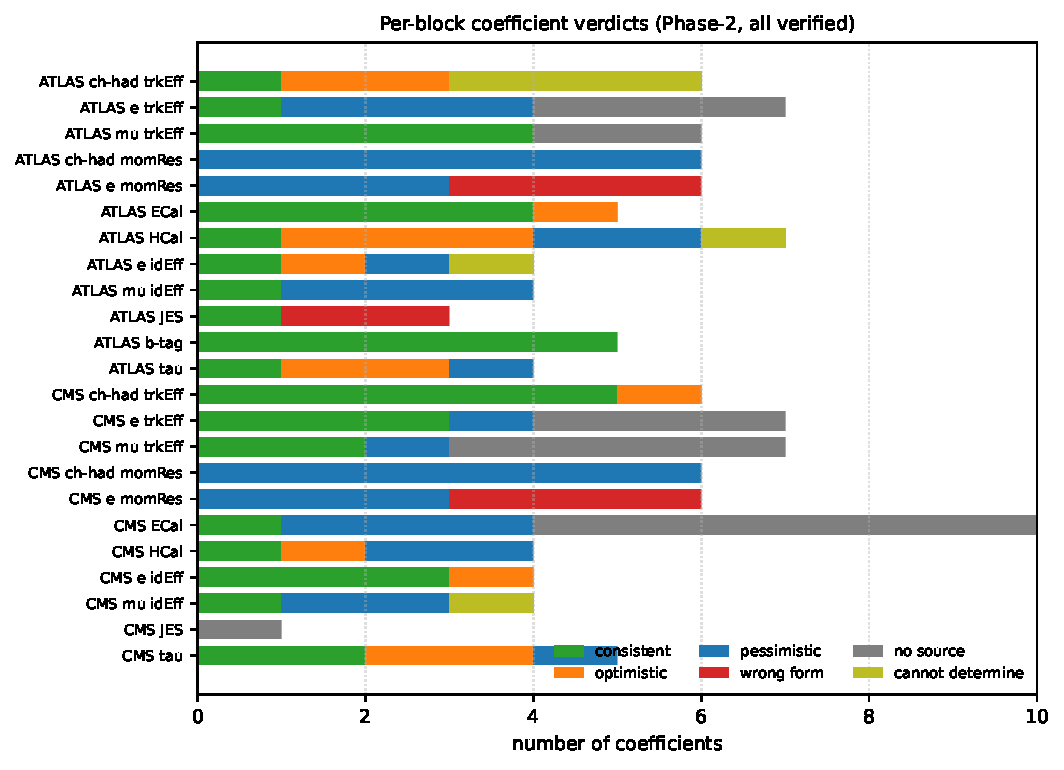
\includegraphics[width=0.92\textwidth]{fig_verdicts.pdf}
\caption{Verdict composition of the measured coefficients, by block, from the
independent verification pass (23 of the 26 blocks; the two photon-identification
and the CMS b-tagging blocks are omitted from this plot but discussed in the text).
``Consistent'' coefficients reproduce their
source; the others carry a proposed source-faithful revision.}
\label{fig:verdicts}
\end{figure}

\begin{longtable}{@{}l l l@{}}
\caption{Per-block verification outcome and headline finding. ``Verdict'' is the
independent verifier's overall judgement.}\label{tab:overview}\\
\toprule
\textbf{Block} & \textbf{Verdict} & \textbf{Headline finding}\\
\midrule
\endfirsthead
\multicolumn{3}{@{}l}{\emph{Table~\ref{tab:overview} continued}}\\
\toprule
\textbf{Block} & \textbf{Verdict} & \textbf{Headline finding}\\
\midrule
\endhead
\bottomrule
\endfoot
\multicolumn{3}{@{}l}{\footnotesize ATLAS card}\\
\midrule
Charged-hadron tracking eff.   & accept$^\ast$ & central plateau $0.95$ optimistic vs.\ measured $\sim$0.86\\
Electron tracking eff.         & accept$^\ast$ & mid-/high-$p_\mathrm{T}$ plateaus pessimistic; low-$p_\mathrm{T}$ unsourced\\
Muon tracking eff.             & accept$^\ast$ & plateaus consistent; low-$p_\mathrm{T}$ floors unsourced\\
Charged-hadron mom.\ res.      & accept$^\ast$ & all six coefficients $\sim$3$\times$ too pessimistic\\
Electron mom.\ res.            & accept$^\ast$ & wrong form: $b\,p_\mathrm{T}$ term is a tracker artefact\\
Muon mom.\ res.\ (pilot)       & accept       & central floor $1.0\%$ optimistic vs.\ $1.7$--$2.3\%$\\
ECal resolution                & \textbf{accept} & $S,C$(FCal) confirmed; only the local $C$ noted\\
HCal resolution                & accept$^\ast$ & central $S$, forward $S/C$ need revision/re-attribution\\
Photon ID eff.                 & accept$^\ast$ & barrel $0.95$ slightly optimistic vs.\ WP $\sim$0.90\\
Electron ID eff.               & accept$^\ast$ & flat $0.95/0.85$ does not match a single WP\\
Muon ID eff.                   & accept$^\ast$ & $0.95$ pessimistic vs.\ modern Medium WP $\sim$0.98\\
Jet energy scale               & accept$^\ast$ & \texttt{ScaleFormula} coefficients unsupported (JER needed)\\
b-tagging                      & accept$^\ast$ & 70\% WP eff.\ + c/light mistag consistent (verified)\\
$\tau$-tagging                 & \textbf{accept} & eff.\ $0.70/0.60$ consistent with Run-2 RNN Medium WP ($0.75/0.60$)\\
\midrule
\multicolumn{3}{@{}l}{\footnotesize CMS card}\\
\midrule
Charged-hadron tracking eff.   & \textbf{accept} & plateau slightly optimistic; otherwise consistent\\
Electron tracking eff.         & accept$^\ast$ & endcap mid-$p_\mathrm{T}$ pessimistic; low-$p_\mathrm{T}$ unsourced\\
Muon tracking eff.             & \textbf{accept} & plateaus consistent; floors/roll-off ad-hoc\\
Charged-hadron mom.\ res.      & accept$^\ast$ & all six coefficients $\sim$3$\times$ too pessimistic\\
Electron mom.\ res.            & accept$^\ast$ & wrong form (tracker copy); $b$ byte-identical to tracker\\
Muon mom.\ res.\ (pilot)       & accept       & barrel floor exact; endcap floor mildly optimistic\\
ECal resolution                & accept$^\ast$ & energy-shape $S,C,N$ disagree; $\eta$-prefactor unsourced\\
HCal resolution                & accept$^\ast$ & central stochastic term too large\\
Photon ID eff.                 & accept$^\ast$ & barrel $0.95$ optimistic vs.\ WP $\sim$0.90\\
Electron ID eff.               & \textbf{accept} & barrel $0.95$ optimistic for reco$\times$loose-ID\\
Muon ID eff.                   & \textbf{accept} & plateaus pessimistic vs.\ Tight/Medium WP\\
Jet energy scale               & \textbf{accept} & generic form; no published source (document as choice)\\
b-tagging                      & \textbf{accept} & CSVM (70\%) WP eff.\ + mistag confirmed vs.\ card's ref\\
$\tau$-tagging                 & accept$^\ast$ & mistag pessimistic vs.\ tight WP; $\eta$ acceptance slightly wide\\
\end{longtable}
{\footnotesize $^\ast$\,\textsc{accept-with-corrections}: verified, with locator/uncertainty refinements that do not reverse the per-coefficient verdicts.}

\subsection{What we learned}
Four findings dominate.

\paragraph{1.~Track momentum resolution is systematically too pessimistic.}
In \emph{both} cards all six charged-hadron coefficients in
Eq.~\ref{eq:momres} are larger than the measured inner-detector / tracker
resolution by a factor $\sim$3. For CMS the source-faithful values
(from~\cite{cms-track}) are $a\!\approx\!0.009,0.015,0.023$ and
$b\!\approx\!2.3,4.2,9.5\times10^{-4}\,\mathrm{GeV^{-1}}$ for the three $\eta$
regions, versus card values $a=0.06,0.10,0.25$ and
$b=1.3,1.7,3.1\times10^{-3}$. The ATLAS card shows the same $\sim$3$\times$
excess against the inner-detector curves of~\cite{atlas-muonres7}
(Figs.~17--18). A caveat the verifier flagged: the cleanest measured anchors are
for muon-ID tracks, so part of the gap may reflect that the card term is meant
to be hadron-specific; this is the one block where we recommend explicit user
review rather than a drop-in replacement. Figure~\ref{fig:momres} shows the gap.

\begin{figure}[H]
\centering
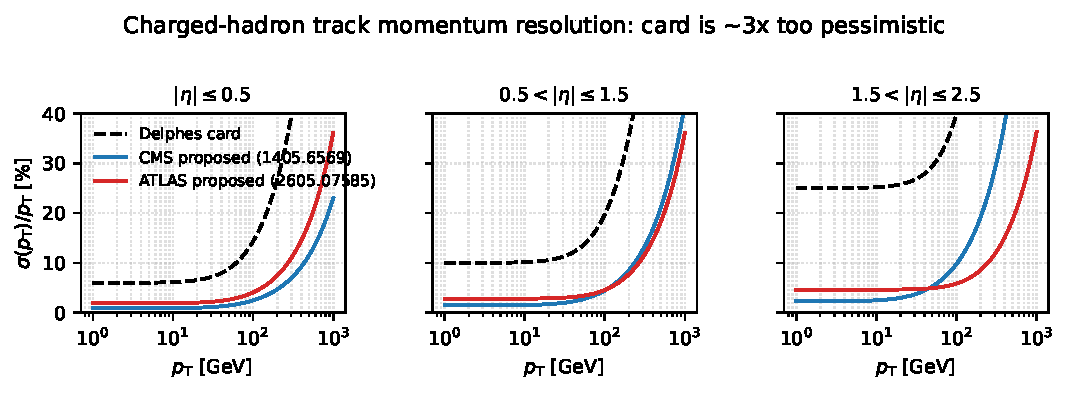
\includegraphics[width=\textwidth]{fig_momres.pdf}
\caption{Charged-hadron track momentum resolution from Eq.~\ref{eq:momres}: the
current card coefficients (dashed) versus the source-faithful values for CMS
(\cite{cms-track}) and ATLAS (\cite{atlas-muonres7}), in the three card $\eta$
regions. The card overestimates the resolution by roughly a factor of three over
most of the $p_\mathrm{T}$ range.}
\label{fig:momres}
\end{figure}

\paragraph{2.~Electron ``momentum'' resolution uses the wrong functional form.}
Electron energy in both ATLAS and CMS is measured by the electromagnetic
calorimeter, whose fractional resolution \emph{improves} with energy, yet the
cards smear electrons with the tracking form of Eq.~\ref{eq:momres}, whose
$b\,p_\mathrm{T}$ term makes the resolution \emph{degrade} linearly with
$p_\mathrm{T}$. The verifiers classify the three $b$ coefficients per card as
\flag{card-wrong}: the term is a copy of the charged-hadron tracker parameters
and must be replaced. The correct form for a calorimeter measurement is
$\sigma(p_\mathrm{T})/p_\mathrm{T}=\sqrt{S^2/p_\mathrm{T}+C^2}$, with a sampling
term $S$ and a constant term $C$. The baseline cards adopt $S=0.101$ (ATLAS EM
barrel test beam~\cite{atlas-ecal}) and $S=0.028$ (CMS ECAL test
beam~\cite{cms-egamma}), with constant terms $C=1.0/1.2/1.8\%$
(ATLAS~\cite{atlas-egammacal}) and $2.0/2.5/5.0\%$ (CMS~\cite{cms-egamma}). This
gives a fractional resolution that \emph{improves} with $p_\mathrm{T}$ (ATLAS
barrel: $\sim$3\% at $10$~GeV $\to\sim$1\% asymptotically); a pure constant term
would instead be optimistic at low $p_\mathrm{T}$. This is the most qualitatively
incorrect block in either card, and is illustrated in Fig.~\ref{fig:eres}: the
card resolution \emph{rises} steeply with $p_\mathrm{T}$, whereas the measured
calorimeter resolution improves with energy.

\begin{figure}[H]
\centering
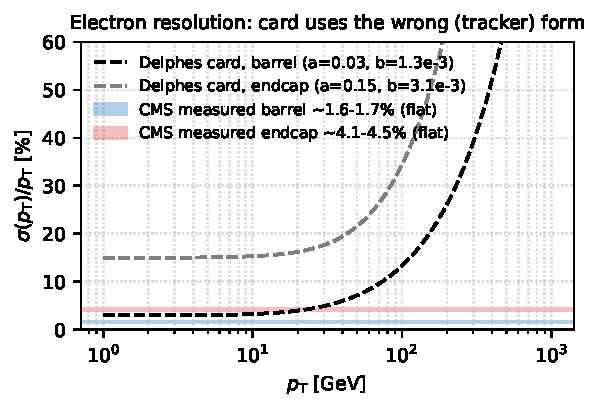
\includegraphics[width=0.62\textwidth]{fig_eres.pdf}
\caption{Electron fractional resolution. The stock card (dashed) applies the
tracking form of Eq.~\ref{eq:momres}, whose $b\,p_\mathrm{T}$ term makes the
resolution \emph{diverge} at high $p_\mathrm{T}$ --- backwards for a calorimeter
measurement. The proposed baseline (solid) uses
$\sqrt{S^2/p_\mathrm{T}+C^2}$, which \emph{improves} with $p_\mathrm{T}$ toward
the constant term $C$, as an EM-calorimeter resolution should.}
\label{fig:eres}
\end{figure}

\paragraph{3.~Several efficiency plateaus are optimistic.}
The ATLAS charged-hadron tracking efficiency plateau of $0.95$ (central) and
$0.85$ (forward) sits above the measured~\cite{atlas-tracking} values of
$\sim$0.86 and $\sim$0.73; the flat $0.95/0.85$ identification efficiencies do
not correspond to any single published working point, and depending on the
intended WP are optimistic (loose-ID plateaus) or pessimistic (Medium/Tight
muon WPs reach $\sim$0.98). These are absolute shifts of $5$--$10\%$ that
directly bias acceptance.

\paragraph{4.~Some blocks are already correct --- and should be locked in.}
The ATLAS electromagnetic-calorimeter resolution ($S=10.1\%\sqrt{\mathrm{GeV}}$,
$C=0.17\%$ local; FCal $S=28.5\%\sqrt{\mathrm{GeV}}$, $C=3.5\%$) is confirmed
against the test-beam and fast-simulation
references~\cite{atlas-ecal,atlas-af3}, and the b-tagging $70\%$ working point
with its c- and light-mistag rates is confirmed against the Run-2 performance
measurement~\cite{atlas-btag}. Recording these as \emph{verified} is as valuable
as flagging the broken ones: it tells a user which numbers they can trust.

\section{Proposed revisions}
Table~\ref{tab:propose} lists the headline source-faithful values for the blocks
where a drop-in revision is well defined. The complete set of $88$ proposed
coefficient changes, each with source, locator, uncertainty, and verifier
verdict, is released in the machine-readable record
(\texttt{run1\_provenance.json}) and the human-readable
\texttt{findings\_summary.md}. Consistent with the project's no-silent-overwrite
rule, the original stock cards are left untouched; the proposed values are instead
emitted into separate \texttt{*\_baseline} (central values) and
\texttt{*\_uncertainty} (per-bin error bands) cards. This first-version (v1) pair
applies the momentum-resolution revisions and the ATLAS charged-hadron tracking
blocks; the efficiency, calorimeter, and tagging revisions are documented but not
yet applied, pending the block-by-block review that the validation overlays
(Appendix~\ref{app:overlays}) support.

\begin{table}[h]
\centering
\caption{Representative proposed revisions (source-faithful central values).
Full list with uncertainties in \texttt{run1\_provenance.json}.}\label{tab:propose}
\begin{tabular}{@{}l l l l@{}}
\toprule
\textbf{Quantity} & \textbf{Region} & \textbf{Card} & \textbf{Proposed}\\
\midrule
\multicolumn{4}{@{}l}{\footnotesize CMS charged-hadron mom.\ res.\ $a$ / $b$~(\,$10^{-4}\,\mathrm{GeV^{-1}}$)}\\
\quad $a,b$ & $|\eta|\!\le\!0.5$   & $0.06,\,13$ & $0.009,\,2.3$\\
\quad $a,b$ & $0.5$--$1.5$         & $0.10,\,17$ & $0.015,\,4.2$\\
\quad $a,b$ & $1.5$--$2.5$         & $0.25,\,31$ & $0.023,\,9.5$\\
\midrule
\multicolumn{4}{@{}l}{\footnotesize Electron mom.\ res.\ $\to\sqrt{S^2/p_\mathrm{T}+C^2}$ ($S,C$); replaces the tracker form}\\
\quad $S,C$ (ATLAS) & $|\eta|\!\le\!0.5$ & $0.03,\,1.3\!\times\!10^{-3}$ & $0.101,\,0.010$\\
\quad $S,C$ (CMS)   & $|\eta|\!\le\!0.5$ & $0.03,\,1.3\!\times\!10^{-3}$ & $0.028,\,0.020$\\
\midrule
\multicolumn{4}{@{}l}{\footnotesize Efficiency plateaus}\\
\quad ATLAS ch.-had.\ track & central, high $p_\mathrm{T}$ & $0.95$ & $0.86$\\
\quad ATLAS ch.-had.\ track & forward, high $p_\mathrm{T}$ & $0.85$ & $0.73$\\
\quad ATLAS muon ID         & $|\eta|\!\le\!1.5$           & $0.95$ & $0.98$ (Medium WP)\\
\quad ATLAS $\tau$ (1-prong)& --                           & $0.70$ & $0.75$ (Run-2 RNN Medium)\\
\midrule
\multicolumn{4}{@{}l}{\footnotesize Calorimeter}\\
\quad CMS HCal $S$ & $|\eta|\!\le\!3.0$ & $1.50$ & $1.10$\\
\bottomrule
\end{tabular}
\end{table}

\section{Validation and limitations}
Three limitations are inherent to a literature-extraction approach and are
recorded with every value. (i)~Many resolution curves are published only as
figures, so the corresponding numbers are \emph{plot-reads} with a
reading uncertainty of order one minor grid division; these are tagged as such.
(ii)~The \textsc{Delphes} $\eta$ binning (boundaries at $0.5,1.5,2.5$) frequently
matches \emph{neither} detector's geometry (ATLAS: $1.05,1.7,2.0$; CMS:
$0.9,1.2,2.4$), so some coefficients are necessarily interpolations across a
boundary rather than a verbatim table value. (iii)~Working-point ambiguity: a
flat efficiency in the card maps to different published numbers depending on the
intended identification WP, which the card does not state; we record the WP we
assumed. (Three CMS blocks --- b-tagging, electron momentum resolution, and
$\tau$-tagging --- lost their verification stage to a workflow interruption and
were re-verified in a separate pass; all three returned \textsc{accept}, so the
record is now complete for all $26$ blocks.)

\section{Conclusion}
A complete provenance pass over the ATLAS and CMS Run-2 \textsc{Delphes} cards is
feasible as a verified, multi-agent literature audit. The pass confirms a number
of card values against their sources and, more importantly, identifies concrete
defects --- a track-momentum resolution too pessimistic by a factor $\sim$3--12
depending on $p_\mathrm{T}$, an electron resolution modelled with the wrong
functional form, and several optimistic efficiency plateaus --- each tied to a
citable measurement and an uncertainty. The deliverables are a machine-readable
provenance file, a human-readable findings summary, first-version
\texttt{*\_baseline} / \texttt{*\_uncertainty} cards, and this manuscript with a
self-validating overlay appendix. Completing the remaining efficiency, calorimeter,
and tagging revisions would let \textsc{Delphes} studies carry a source-traceable
detector-modelling systematic derived directly from the per-bin uncertainty bands.

\appendix
\section{Validation of figure-read parameterizations}
\label{app:overlays}
Several parameterizations are read from published performance figures rather than
from a numeric table. To document that each extraction is faithful, we overlay the
adopted \textsc{Delphes} curve (with its uncertainty band) directly on the source
figure --- so the reader can verify the agreement by eye, and so a mis-extraction
is caught immediately. Where the source figure is published in an arXiv paper we
draw on the rendered figure itself (Figs.~\ref{fig:ovl-cmsmu}--\ref{fig:ovl-cmstrk});
for ATLAS auxiliary figures we overlay on the digitized points, citing the figure
(Fig.~\ref{fig:ovl-atlastrk}). Each panel reproduces the published figure under our
curve; the band is the per-bin systematic used in the \texttt{*\_uncertainty} card.

\begin{figure}[h]
\centering
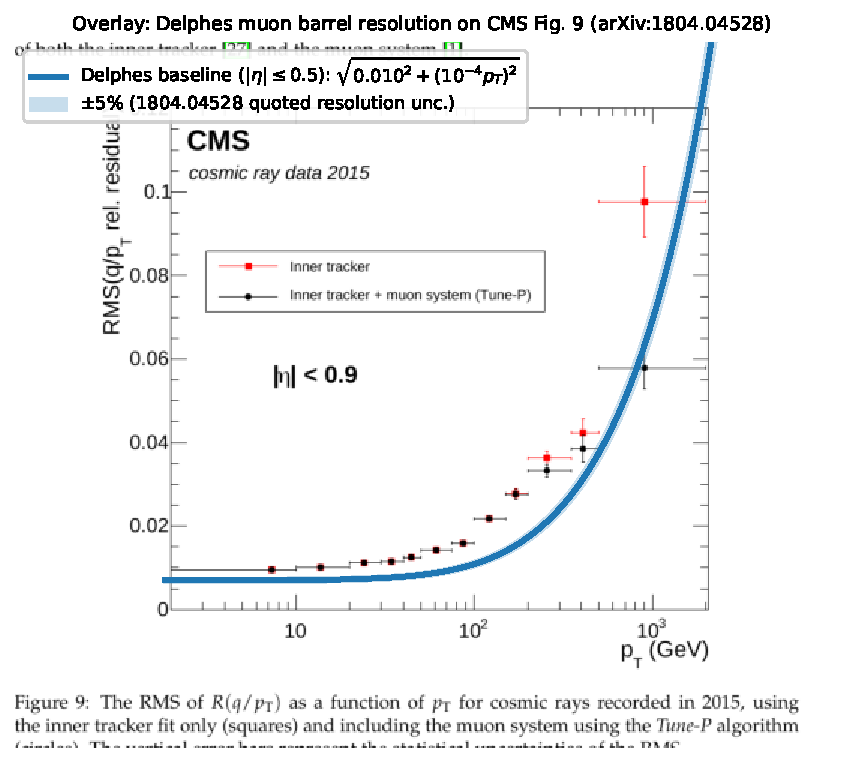
\includegraphics[width=0.49\textwidth]{aux_overlay_onfigure_muon.pdf}\hfill
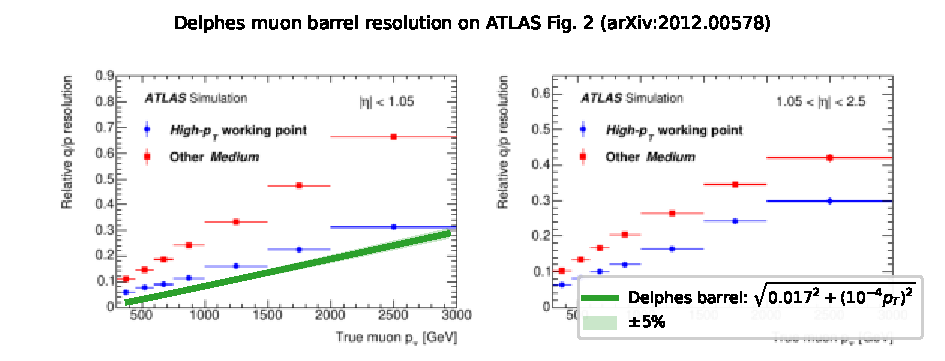
\includegraphics[width=0.49\textwidth]{aux_overlay_onfigure_atlasmu.pdf}
\caption{Muon momentum resolution. Left: \textsc{Delphes} CMS barrel curve on CMS
Fig.~9~\cite{cms-muon} (RMS of $R(q/p_\mathrm{T})$, $|\eta|<0.9$, cosmic rays); the
card is compared to the \emph{inner-tracker-only} points --- CMS high-$p_\mathrm{T}$
muons combine the muon system (Tune-P, $\sim$6\% at $1$~TeV vs.\ the tracker's
$\sim$10\%), so a single-Gaussian card tuned to the tracker points is conservative
at high $p_\mathrm{T}$. Right: \textsc{Delphes} ATLAS barrel curve on ATLAS
Fig.~2~\cite{atlas-muon13fullrun2} ($q/p$ resolution vs.\ $p_\mathrm{T}$,
$|\eta|<1.05$; the endcap panel is shown for context, not overlaid).}
\label{fig:ovl-cmsmu}
\end{figure}

\begin{figure}[h]
\centering
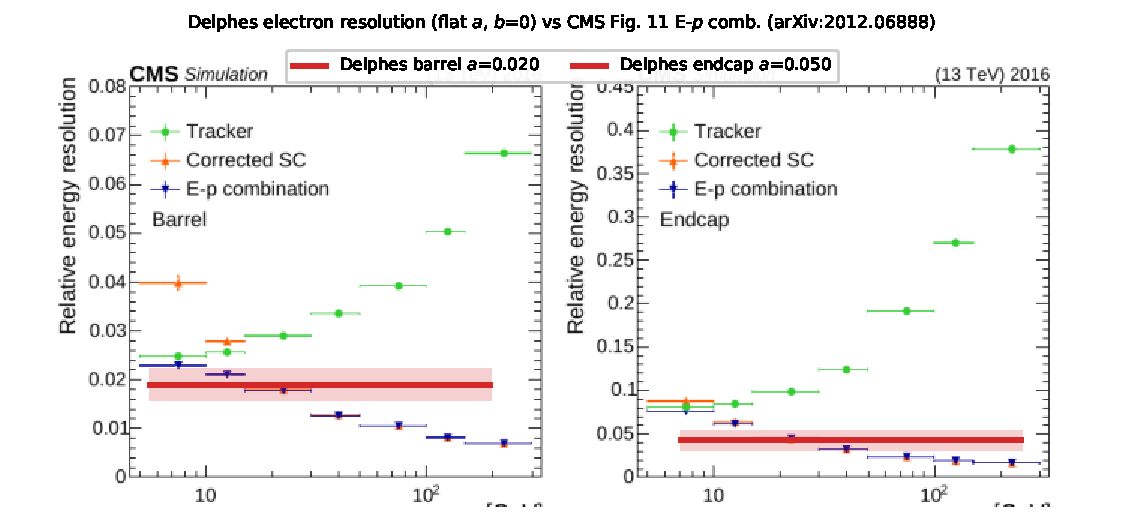
\includegraphics[width=0.62\textwidth]{aux_overlay_onfigure_cmsel.pdf}
\caption{Electron resolution: the flat \textsc{Delphes} constant term ($b=0$) on
CMS Fig.~11~\cite{cms-egamma} (barrel/endcap relative energy resolution vs.\
$p_\mathrm{T}$). Our value matches the E-$p$ combination at low/intermediate
$p_\mathrm{T}$ and is conservative at high $p_\mathrm{T}$, where the calorimeter
resolution improves.}
\label{fig:ovl-cmsel}
\end{figure}

\begin{figure}[h]
\centering
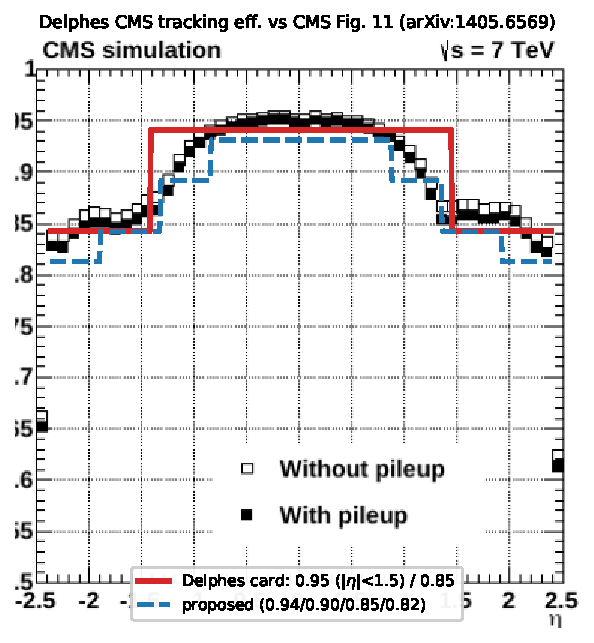
\includegraphics[width=0.55\textwidth]{aux_overlay_onfigure_cmstrkeff.pdf}
\caption{CMS charged-hadron tracking efficiency vs.\ $\eta$ on CMS
Fig.~11~\cite{cms-track}: the card step ($0.95/0.85$) and the proposed finer
binning, both bracketing the measured plateau and forward fall-off.}
\label{fig:ovl-cmstrk}
\end{figure}

\begin{figure}[h]
\centering
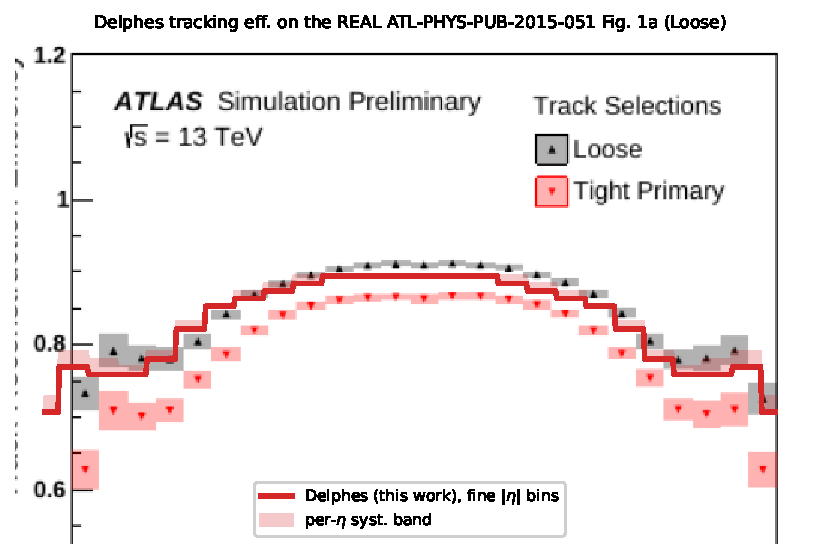
\includegraphics[width=0.52\textwidth]{aux_overlay_onfigure_atlastrkeff.pdf}\hfill
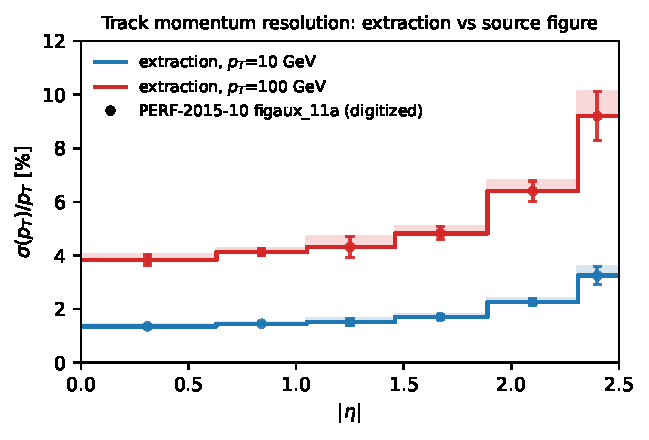
\includegraphics[width=0.46\textwidth]{aux_momres_overlay.pdf}
\caption{ATLAS charged-hadron tracking blocks. Left: \textsc{Delphes} tracking
efficiency (fine $|\eta|$ bins) on the real ATL-PHYS-PUB-2015-051 Fig.~1a (Loose
selection) --- the curve tracks the published points across $\eta$. Right: track
momentum resolution vs.\ $\eta$ (overlay on digitized points; the source auxiliary
figure was not directly retrievable). Remaining blocks (muon/photon identification)
are validated by the consistency arguments in the text (the muon plateaus of
$\sim$0.99/0.95 make the card's flat $0.95$ conservative).}
\label{fig:ovl-atlastrk}
\end{figure}

\begin{figure}[h]
\centering
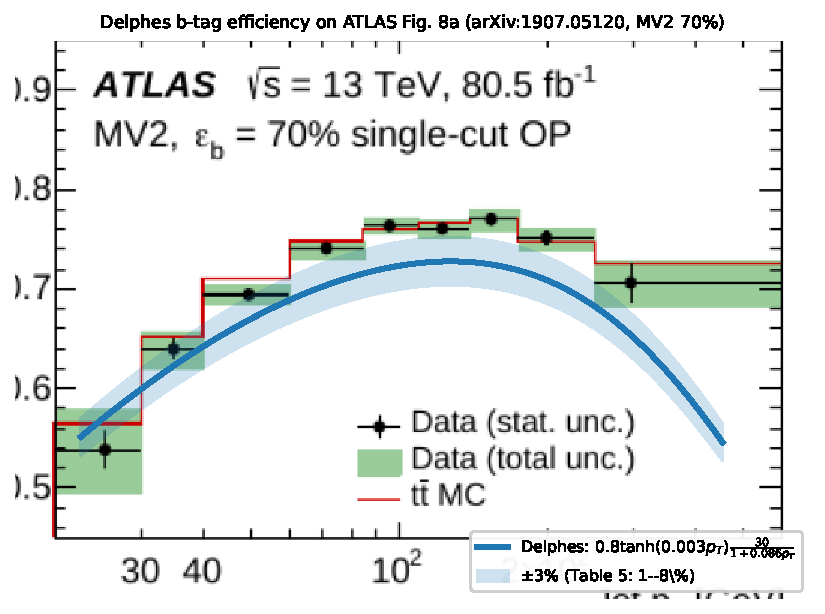
\includegraphics[width=0.52\textwidth]{aux_overlay_onfigure_atlasbtag.pdf}\hfill
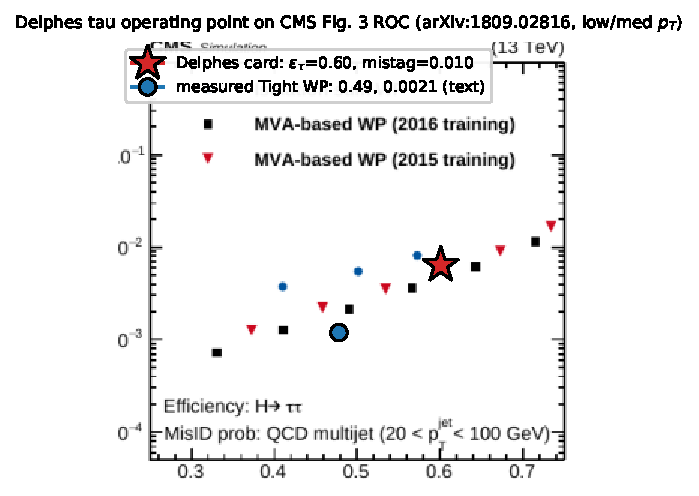
\includegraphics[width=0.46\textwidth]{aux_overlay_onfigure_cmstau.pdf}
\caption{Flavour tagging. Left: \textsc{Delphes} $b$-tagging efficiency on ATLAS
Fig.~8a~\cite{atlas-btag} (MV2 $\varepsilon_b=70\%$); the card matches at low
$p_\mathrm{T}$ but falls off too steeply at high $p_\mathrm{T}$ (a tuning target).
Right: the card $\tau$ operating point ($\varepsilon_\tau=0.6$, mistag $=0.01$) on
the CMS misidentification-vs-efficiency ROC, Fig.~3~\cite{cms-tau}; the card point
lies \emph{above} the measured MVA curve --- the flat $0.01$ mistag is a factor
$\sim$2--3 larger than the measured value at $\varepsilon_\tau=0.6$, i.e.\ the card
is conservative (pessimistic) on the $\tau$ mistag rate.}
\label{fig:ovl-tag}
\end{figure}

\begin{figure}[h]
\centering
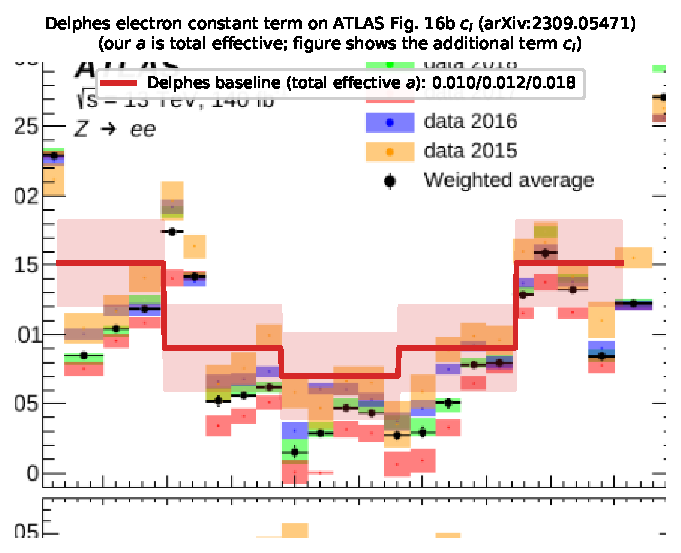
\includegraphics[width=0.52\textwidth]{aux_overlay_onfigure_atlasel.pdf}\hfill
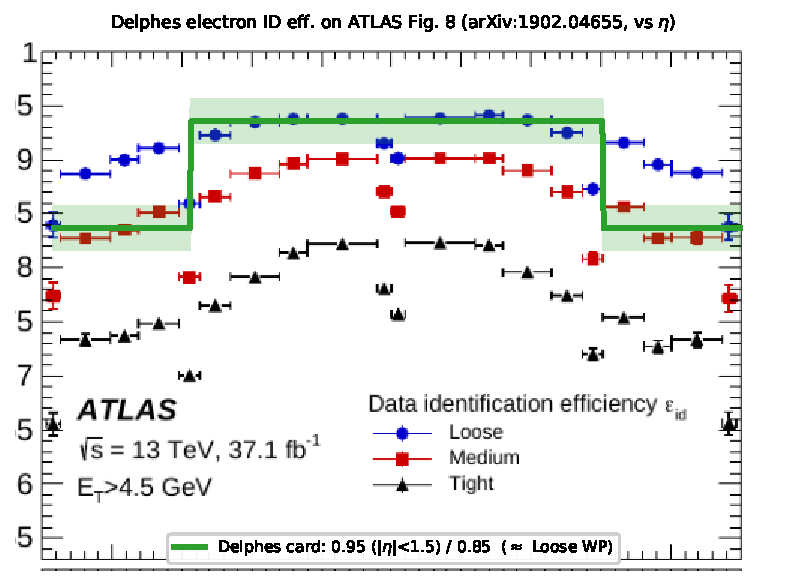
\includegraphics[width=0.46\textwidth]{aux_overlay_onfigure_atlaseid.pdf}
\caption{ATLAS electron. Left: the \textsc{Delphes} electron constant term on the
additional-constant-term $c_i(\eta)$ of Fig.~16b~\cite{atlas-egammacal} (our $a$ is
the total effective term, so it brackets $c_i$ from above and follows the same
$\eta$ structure). Right: \textsc{Delphes} electron identification efficiency on
ATLAS Fig.~8~\cite{atlas-egamma} (vs.\ $\eta$); the card $0.95/0.85$ is closest to
the Loose working point, but does not match a single published WP --- it is
slightly optimistic centrally (Loose plateau $\sim$0.93) and pessimistic in the
endcap ($\sim$0.90).}
\label{fig:ovl-atlasel}
\end{figure}

\begin{figure}[h]
\centering
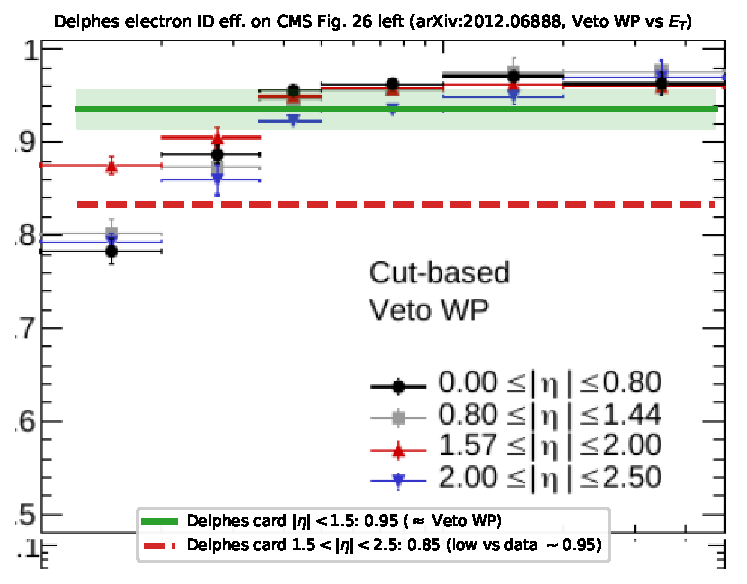
\includegraphics[width=0.49\textwidth]{aux_overlay_onfigure_cmseid.pdf}\hfill
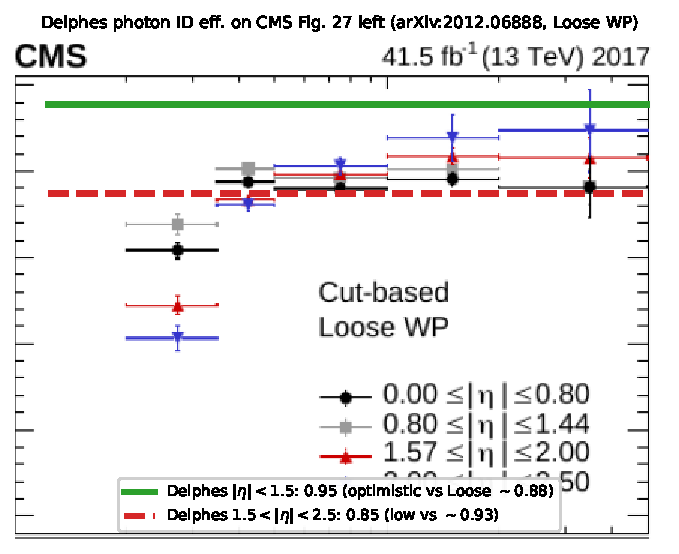
\includegraphics[width=0.49\textwidth]{aux_overlay_onfigure_cmsphot.pdf}
\caption{CMS electron (left) and photon (right) identification efficiency on CMS
Figs.~26 and~27~\cite{cms-egamma} (cut-based working points vs.\ $E_\mathrm{T}$,
four $\eta$ ranges). For electrons the card central $0.95$ matches the Veto
plateau while the forward $0.85$ is too pessimistic (measured $\sim$0.95). For
photons the card central $0.95$ is mildly optimistic (Loose plateau $\sim$0.88)
and the forward $0.85$ low (measured $\sim$0.93) --- both flagged for tuning.}
\label{fig:ovl-cmseid}
\end{figure}

\begin{thebibliography}{99}
\small
\bibitem{delphes} J.~de Favereau \emph{et al.} (DELPHES~3 Collaboration),
  ``DELPHES~3: a modular framework for fast simulation of a generic collider
  experiment,'' JHEP \textbf{02} (2014) 057, arXiv:1307.6346.
\bibitem{atlas-muonres7} ATLAS Collaboration, ``Measurement of the muon
  reconstruction performance of the ATLAS detector using 2010 LHC $pp$ collision
  data at $\sqrt{s}=7$~TeV,'' Eur.\ Phys.\ J.\ C \textbf{74} (2014) 3034,
  arXiv:1404.4562.
\bibitem{atlas-muon13} ATLAS Collaboration, ``Muon reconstruction performance of
  the ATLAS detector in $pp$ collision data at $\sqrt{s}=13$~TeV,'' Eur.\ Phys.\
  J.\ C \textbf{76} (2016) 292, arXiv:1603.05598.
\bibitem{atlas-muon13fullrun2} ATLAS Collaboration, ``Muon reconstruction and
  identification efficiency in ATLAS using the full Run~2 $pp$ collision data set
  at $\sqrt{s}=13$~TeV,'' Eur.\ Phys.\ J.\ C \textbf{81} (2021) 578,
  arXiv:2012.00578.
\bibitem{cms-muon} CMS Collaboration, ``Performance of the CMS muon detector and
  muon reconstruction with proton-proton collisions at $\sqrt{s}=13$~TeV,''
  JINST \textbf{13} (2018) P06015, arXiv:1804.04528.
\bibitem{cms-track} CMS Collaboration, ``Description and performance of track and
  primary-vertex reconstruction with the CMS tracker,'' JINST \textbf{9} (2014)
  P10009, arXiv:1405.6569.
\bibitem{atlas-tracking} ATLAS Collaboration, ``Charged-particle distributions
  in $\sqrt{s}=13$~TeV $pp$ interactions measured with the ATLAS detector,''
  Phys.\ Lett.\ B \textbf{758} (2016) 67, arXiv:1602.01633.
\bibitem{cms-egamma} CMS Collaboration, ``Electron and photon reconstruction and
  identification with the CMS experiment at the CERN LHC,'' JINST \textbf{16}
  (2021) P05014, arXiv:2012.06888. (Run-2, 13~TeV; replaces the Run-1
  arXiv:1502.02701.)
\bibitem{atlas-egamma} ATLAS Collaboration, ``Electron reconstruction and
  identification in the ATLAS experiment using the 2015 and 2016 LHC $pp$
  collision data at $\sqrt{s}=13$~TeV,'' Eur.\ Phys.\ J.\ C \textbf{79} (2019)
  639, arXiv:1902.04655.
\bibitem{atlas-egammacal} ATLAS Collaboration, ``Electron and photon energy
  calibration with the ATLAS detector using LHC Run~2 data,'' JINST \textbf{19}
  (2024) P02009, arXiv:2309.05471. (Run-2 electron resolution.)
\bibitem{atlas-ecal} M.~Aharrouche \emph{et al.} (ATLAS Electromagnetic Barrel
  Calorimeter Collaboration), ``Energy linearity and resolution of the ATLAS
  electromagnetic barrel calorimeter in an electron test-beam,'' Nucl.\ Instrum.\
  Meth.\ A \textbf{568} (2006) 601, arXiv:physics/0608012.
\bibitem{atlas-af3} ATLAS Collaboration, ``AtlFast3: the next generation of fast
  simulation in ATLAS,'' Comput.\ Softw.\ Big Sci.\ \textbf{6} (2022) 7,
  arXiv:2109.02551.
\bibitem{atlas-btag} ATLAS Collaboration, ``ATLAS b-jet identification
  performance and efficiency measurement with $t\bar t$ events in $pp$
  collisions at $\sqrt{s}=13$~TeV,'' Eur.\ Phys.\ J.\ C \textbf{79} (2019) 970,
  arXiv:1907.05120.
\bibitem{cms-btag} CMS Collaboration, ``Identification of heavy-flavour jets with
  the CMS detector in $pp$ collisions at $13$~TeV,'' JINST \textbf{13} (2018)
  P05011, arXiv:1712.07158.
\bibitem{cms-tau} CMS Collaboration, ``Performance of reconstruction and
  identification of $\tau$ leptons decaying to hadrons and $\nu_\tau$ in $pp$
  collisions at $\sqrt{s}=13$~TeV,'' JINST \textbf{13} (2018) P10005,
  arXiv:1809.02816.
\bibitem{cms-jes} CMS Collaboration, ``Jet energy scale and resolution in the CMS
  experiment in $pp$ collisions at $8$~TeV,'' JINST \textbf{12} (2017) P02014,
  arXiv:1607.03663.
\bibitem{atlas-jes} ATLAS Collaboration, ``Jet energy scale measurements and
  their systematic uncertainties in $pp$ collisions at $\sqrt{s}=13$~TeV with the
  ATLAS detector,'' Phys.\ Rev.\ D \textbf{96} (2017) 072002, arXiv:1703.09665.
\end{thebibliography}

\end{document}
